%\documentclass[11pt]{article}
%\usepackage{fullpage}
%\usepackage{graphicx}

%\begin{document}

\subsection{Product perspective}
The TrackMe software-based service, Data4Help, has  other two services built on its top: AutomatedSOS and Track4Run. These two services exploit Data4Help's features, resources and links to external services. Not all the system's tasks in fact are provided only by the application: maps or payment services are committed to external systems. The application provides some services also for users who install it on a non-weareble device, but it mainly exploits weareble devices' features for all the three services. They are indeed based on health and location features that must be updated in real-time. \newline

A view of the relations that intervene among concepts that will be at the base of the system is given by the following diagram.

\begin{center}
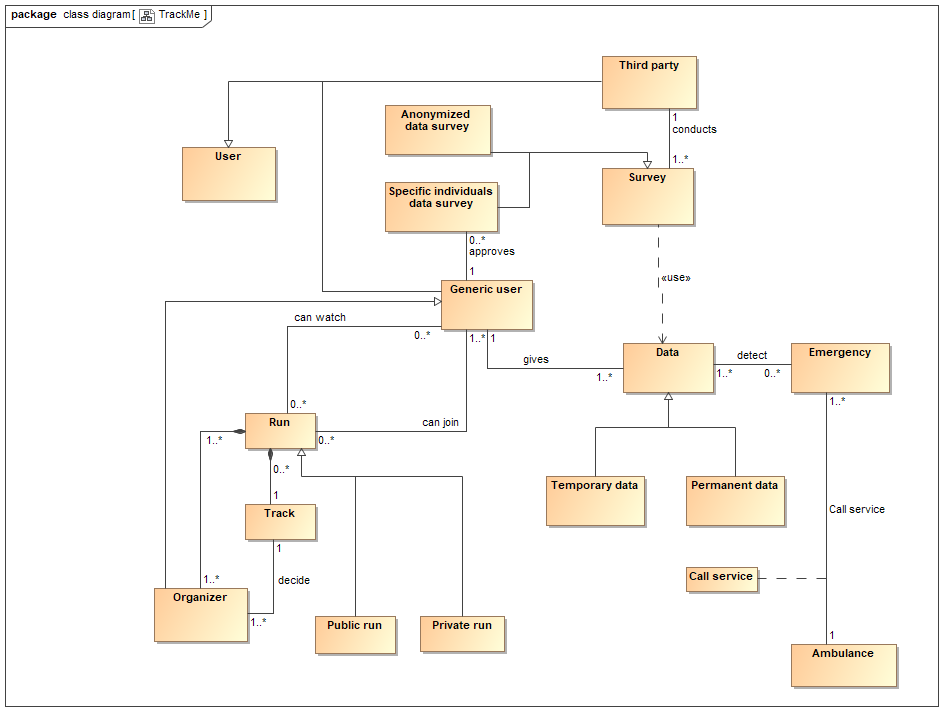
\includegraphics[scale=0.5]{sections/diagrams/class_diagram.png}
\end{center}

A central role is performed by the generic user and by data that can tell him/her and third parties about his/her status. Besides data management (with a semi-passive role for the generic user), the application is about running races and it allows generic users to enter in contact with each other watching or organizing them. Finally, we can see different types of data, races and surveys, that requires different interactions with users.

As the running race management is one of the most complex services among those offered to be understood in its phases, here's a specification of them.

\begin{center}
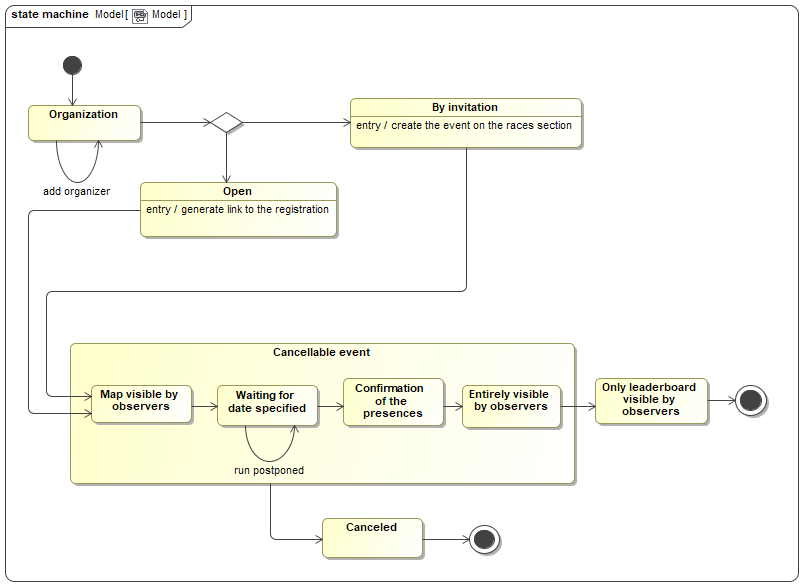
\includegraphics[scale=0.6]{sections/diagrams/stateDiagram.png}
\end{center}

In order to know how to behave consequently to the organization form filling, it is required to indicate if the running race will be open or by invitation. After this first part the run enters in a state in which it is allowed to cancel it until it's end is reached.

\subsection{Product functions}
The requirements of all services dealt with above can be grouped in the following system's main functions.

\subsubsection{Data collection and updating}
This function is the one on which is based Data4Help service and that is exploited by the other two services. For a generic user (not a third party), data are collected through a form during the registration phase and subsequently through automatic update.

This takes place through the sensors and the GPS system of the wearable device on which the service is active, which update the health status and position of the user. These data collected in real-time are the ones that AutomatedSOS needs (if the user is subscribed at it) to call for help if the user's health is in a state of emergency. Data inherent only to localization will be instead fundamental to allow the service Run4Track to let other users follow the runners' movements during the race.

\subsubsection{Data exchange with external entities}
Complementary to the previous one, this function deals with the management of those aspects that affect third parties and those that allow completing AutomatedSOS service.

Data4Help is in fact thought to give a service to third parties: companies, research institutes, and whatever entity could be interested in getting hold of data of a person for some reason (such as leading surveys or sending specific advertising to some groups of people). Third parties, after being adequately identified through a code agreed with the company TrackMe, can obtain two types of data from the service: specific individuals ones or anonymized ones.

In order to obtain data of specific individuals, in which the survey's object can be considered identifiable, a third party can search through a search dialog or filters an individual or a group of fewer than 1000 persons. Then, Data4Help creates a request for use of data that the interested users will receive as a notification. Only after receiving their consent Data4Help will allow the third party to receive those data, updated from time to time.

If the third party wants to lead an anonymized survey instead, the application doesn't need the users' consent and it gives automatically data of groups of users of more than 1000 persons.

Regarding AutomatedSOS, once a situation of emergency is ascertained, the application is capable, thanks to the data collected and the agreement with emergency services in Europe and USA, of providing an immediate and accurate help service. 

\subsubsection{Run management} 
Here "management" is intended to indicate the management of a running race led by a user, who is allowed by the application to organize it and update its status. In fact, the user is able to organize a new race through a form and an external map service.

The organizer can optionally indicate in the form other organizers, who will help in the race management, once the initial phase of race profiling is completed. After the event is created, every organizer has the possibility to postpone the race before its begin and to cancel it before its end. Other two actions can be performed by the organizers: sign a runner as "present" at the race and as "disqualified" with respect to its rules. Those two actions can be very useful to be performed by several persons, especially during races of certain dimensions. Furthermore, those flags will be fundamental for the race monitoring of other users.

During the form compilation, the user has to specify if the race will be open or by invitation, in order to create respectively the public announcement or private links to a registration form.
 
\subsubsection{Data monitoring and consequent actions on them}

The generic user, daily opening the application finds immediately his/her data recorded through the wearable device and notifications (such as the request of data sharing from a company). Naturally, the user can answer the notification as far as required. In another section that can be found through the menù, the user can monitor races to whom he/she subscribed or which are organized by him/her, and next to it he/she finds a list of races in neatness and time order. There the user can subscribe to a race or watch it in real-time.

The display of the race takes place through maps provided by external services and on the shown path there are markers associated with runners signed as "present". On the screen, there's also a leaderboard with the runners' names associated with the markers through a number. It is visible if a runner is disqualified (the marker is blocked where he/she was disqualified and the name is grey).
 
\subsection{User characteristics}
The system has the following actors:
\begin{itemize}
\item \textbf{Generic user}: a person who has a user account through which he/she monitors his/her data and can subscribe to services for emergency automated calls and for joining running races, as well as organizing them.
\item \textbf{Third party}: a company or association registered agent who can ask for groups' or individuals' data.
\item \textbf{Administrator}: A TrackMe employee who can make some changes in the forms other actors have to compile.
\end{itemize}

\subsection{Assumptions, dependencies and constraints}
[D1] - Third parties own an alphanumerical code received from a TrackMe administrator used to verify their identities and match them with the company account. \newline

\hspace{-\parindent}[D2] - Device sensors can provide accurate data to the app. \newline

\hspace{-\parindent}[D3] - TrackMe is affiliated with NUE 112 (Numero Unico per le Emergenze) to offer assistance in Europe, and with 911 to offer assistance in the USA. \newline

\hspace{-\parindent}[D4] - The run can be joined only by persons enrolled through the app. \newline

\hspace{-\parindent}[D5] - If it is required a payment to enroll a run, an external service will guarantee secure transactions and receipts by e-mail. \newline

%\end{document}